\chapter{\section{Methodology}{{\normalfont\fontsize{14}{16}\bfseries}}
This chapter discusses the risk assessment tool used for Artificial intelligence integration in robotics. The tool we use here is Failure Mode Effect Analysis with an extension of System Theory Process Analysis. 
%Since no known standards exist in the market for AI integration in robotics, we use FMEA-STPA as a tool for risk assessment and try to identify the failures and risk related. 
In light of the absence of established standards within the industries and market, we use FMEA-STPA as a tool for conducting risk assessment for the AI integration in robotics, this would help to identify and mitigate the potential failures and associated risks.
The identified potential failures are similar to the data of the Autonomous Driving system. We use FMEA-STPA on perception-based grasping in robots. Since it is one of the best-known scenarios where robots make use of Artificial intelligence and do manipulation tasks. The reason for selecting FMEA and adding an extension of STPA for the risk assessment and the basic definitions of the terms used in processes are explained. The system setup and the boundary conditions are explained in a subsection of the chapter. The use case from which the results are manipulated is also explained along with its relevance.

\subsection{\RaggedRight Robot Bin Picking Application as an Industrial Use Case for the Perception-based Grasping }

In an ideal smart system where robots and humans work together, tasks are split into different jobs, each with smaller tasks. For example, imagine a situation where robots and people team up to pick warehouse parts, put them together a bit, and then move the assembled kits. Some tasks need both humans and robots to work together, while others need each to do their own thing. Besides the main tasks, there are other jobs like fixing problems, figuring out issues, learning new things, giving or getting instructions, handling changes, and planning what to do. Everyone in the system has to work together in these tasks, and sometimes there might be risky situations. %edited by cg

The bin-picking robot system is a highly advanced automation solution designed for the efficient picking and placing of machined parts from two adjacent heavy boxes onto a conveyor belt. This fixed robotic system incorporates cutting-edge technologies, including a magnetic gripper with a spring mechanism that allows robust picking, an RGB-D camera for precise object identification, and Safe Human Detection sensors for human presence detection.

\subsubsection{System Components}

Robot Arm: The robot arm is securely fixed on a stationary base which is a versatile and powerful solution for handling tasks with precision. With a strong payload capacity of 12-14 kg and an extensive reach of 1400 mm, it's well-equipped for various industrial applications. What makes it stand out is its intelligent head, which cleverly integrates Lidar sensors and an RGB-D camera directly into the arm's seventh axis. Unlike traditional setups, this design enhances the arm's flexibility by seamlessly incorporating advanced sensing capabilities. With seven degrees of freedom, it can move precisely in complex tasks, adapting to different orientations. Plus, it's built tough with an IP 65 rating, ensuring resilience against dust and water—perfect for challenging industrial settings. The intelligent head's Lidar sensors enable real-time 3D mapping, helping the arm navigate and plan its path effectively. The integrated RGB-D camera adds high-resolution color imagery and depth perception, making it adept at recognizing objects and handling them precisely. This robotic arm finds applications in manufacturing, assembly lines, logistics, and research and development tasks. Its adaptability, combined with a robust IP 65 rating, makes it a game-changer for organizations seeking advanced automation solutions. Equipped with a magnetic gripper as an end effector for robust and adaptable picking.

Magnetic Gripper: Features a spring mechanism for smooth and secure picking of machined parts.
The magnetic force ensures a strong grip on objects, preventing unintentional drops.

RGB-D Camera: Mounted on the robot arm for comprehensive color (RGB) and depth (D) information.
Utilized for the identification of both the box and the machined parts within it.

Safe Human Detection Sensors: Integrated into the system to identify the presence of humans in the operational vicinity. Provides real-time feedback for safety and operational considerations.

External PLC: The Programmable Logic Controller integrated into the system is used for the human-robot interaction addition to the graphical user interface.

Conveyor Belt: The conveyor belt is placed within reach of the robot arm, to place the object picked from the box. The conveyor belt moves the placed workpiece to the next workstation.

Control System: Manages the overall operation of the robot system and receives input from the RGB-D camera and Safe Human Detection sensors, This System controls the actions of the robot arm, magnetic gripper, and conveyor belt.

The heart of the robotic system lies within a sleek and efficient modular control box. This compact unit seamlessly combines the power of Artificial Intelligence (AI), safety protocols, motion control, and power management. The modular design streamlines the control processes, ensuring a harmonious interaction between these vital components. With AI, the robotic arm gains intelligent decision-making capabilities, adapting to various scenarios. The safety module prioritizes secure operations, and the motion control module enables precise and fluid movements. Simultaneously, the power module efficiently manages energy distribution for a reliable and continuous power supply. This modular control box represents the central intelligence that propels our cutting-edge robotic arm, ensuring optimal performance across a spectrum of applications.

\subsubsection{Operational Sequence}

1. Start-Up: Power on the entire system, including the robot arm, magnetic gripper, RGB-D camera, and Safe Human Detection sensors, Initiate the control system for seamless operation.

2. Picking Phase: The robot arm starts picking machined parts from the first box using the magnetic gripper.

3. Object and Box Identification: The RGB-D camera identifies the box and the machined parts within it with high precision, Safe Human Detection sensors continuously monitor the surroundings for the presence of humans.

4. Orientation Check: The system checks the orientation of the picked object. If incorrect, the robot attempts a re-pick, allowing for up to two failures before corrective actions.

5. Lookup Point and Scene Re-identification: If more than two failures occur, the robot moves to a lookup point.The RGB-D camera re-identifies the box and machined parts, correcting orientation information.

6. Cycle Management: After successfully completing five operational cycles, the system triggers a return to the lookup point.This periodic lookup adapts the system to potential changes in the scene within the box.

7. Human Intervention for Bin Replacement: When the first box is empty, the robot sends a signal for human intervention. A human operator replaces the empty box with a filled one.

8. Placement and Conveyor Belt: The robot continues picking from the second box and places machined parts on a conveyor belt. The robot changes its orientation to keep the time and avoid singularity errors during pick and place from the second box.

9. Specific Placement: The robot is programmed to place objects precisely in a predefined location. The magnetic gripper ensures a controlled release, preventing unintended drops.

10. End of Cycle:The operational cycle completes within the designated 28-second timeframe.

\begin{figure}
    \centering
    \begin{minipage}{0.8\linewidth}
    \centering
        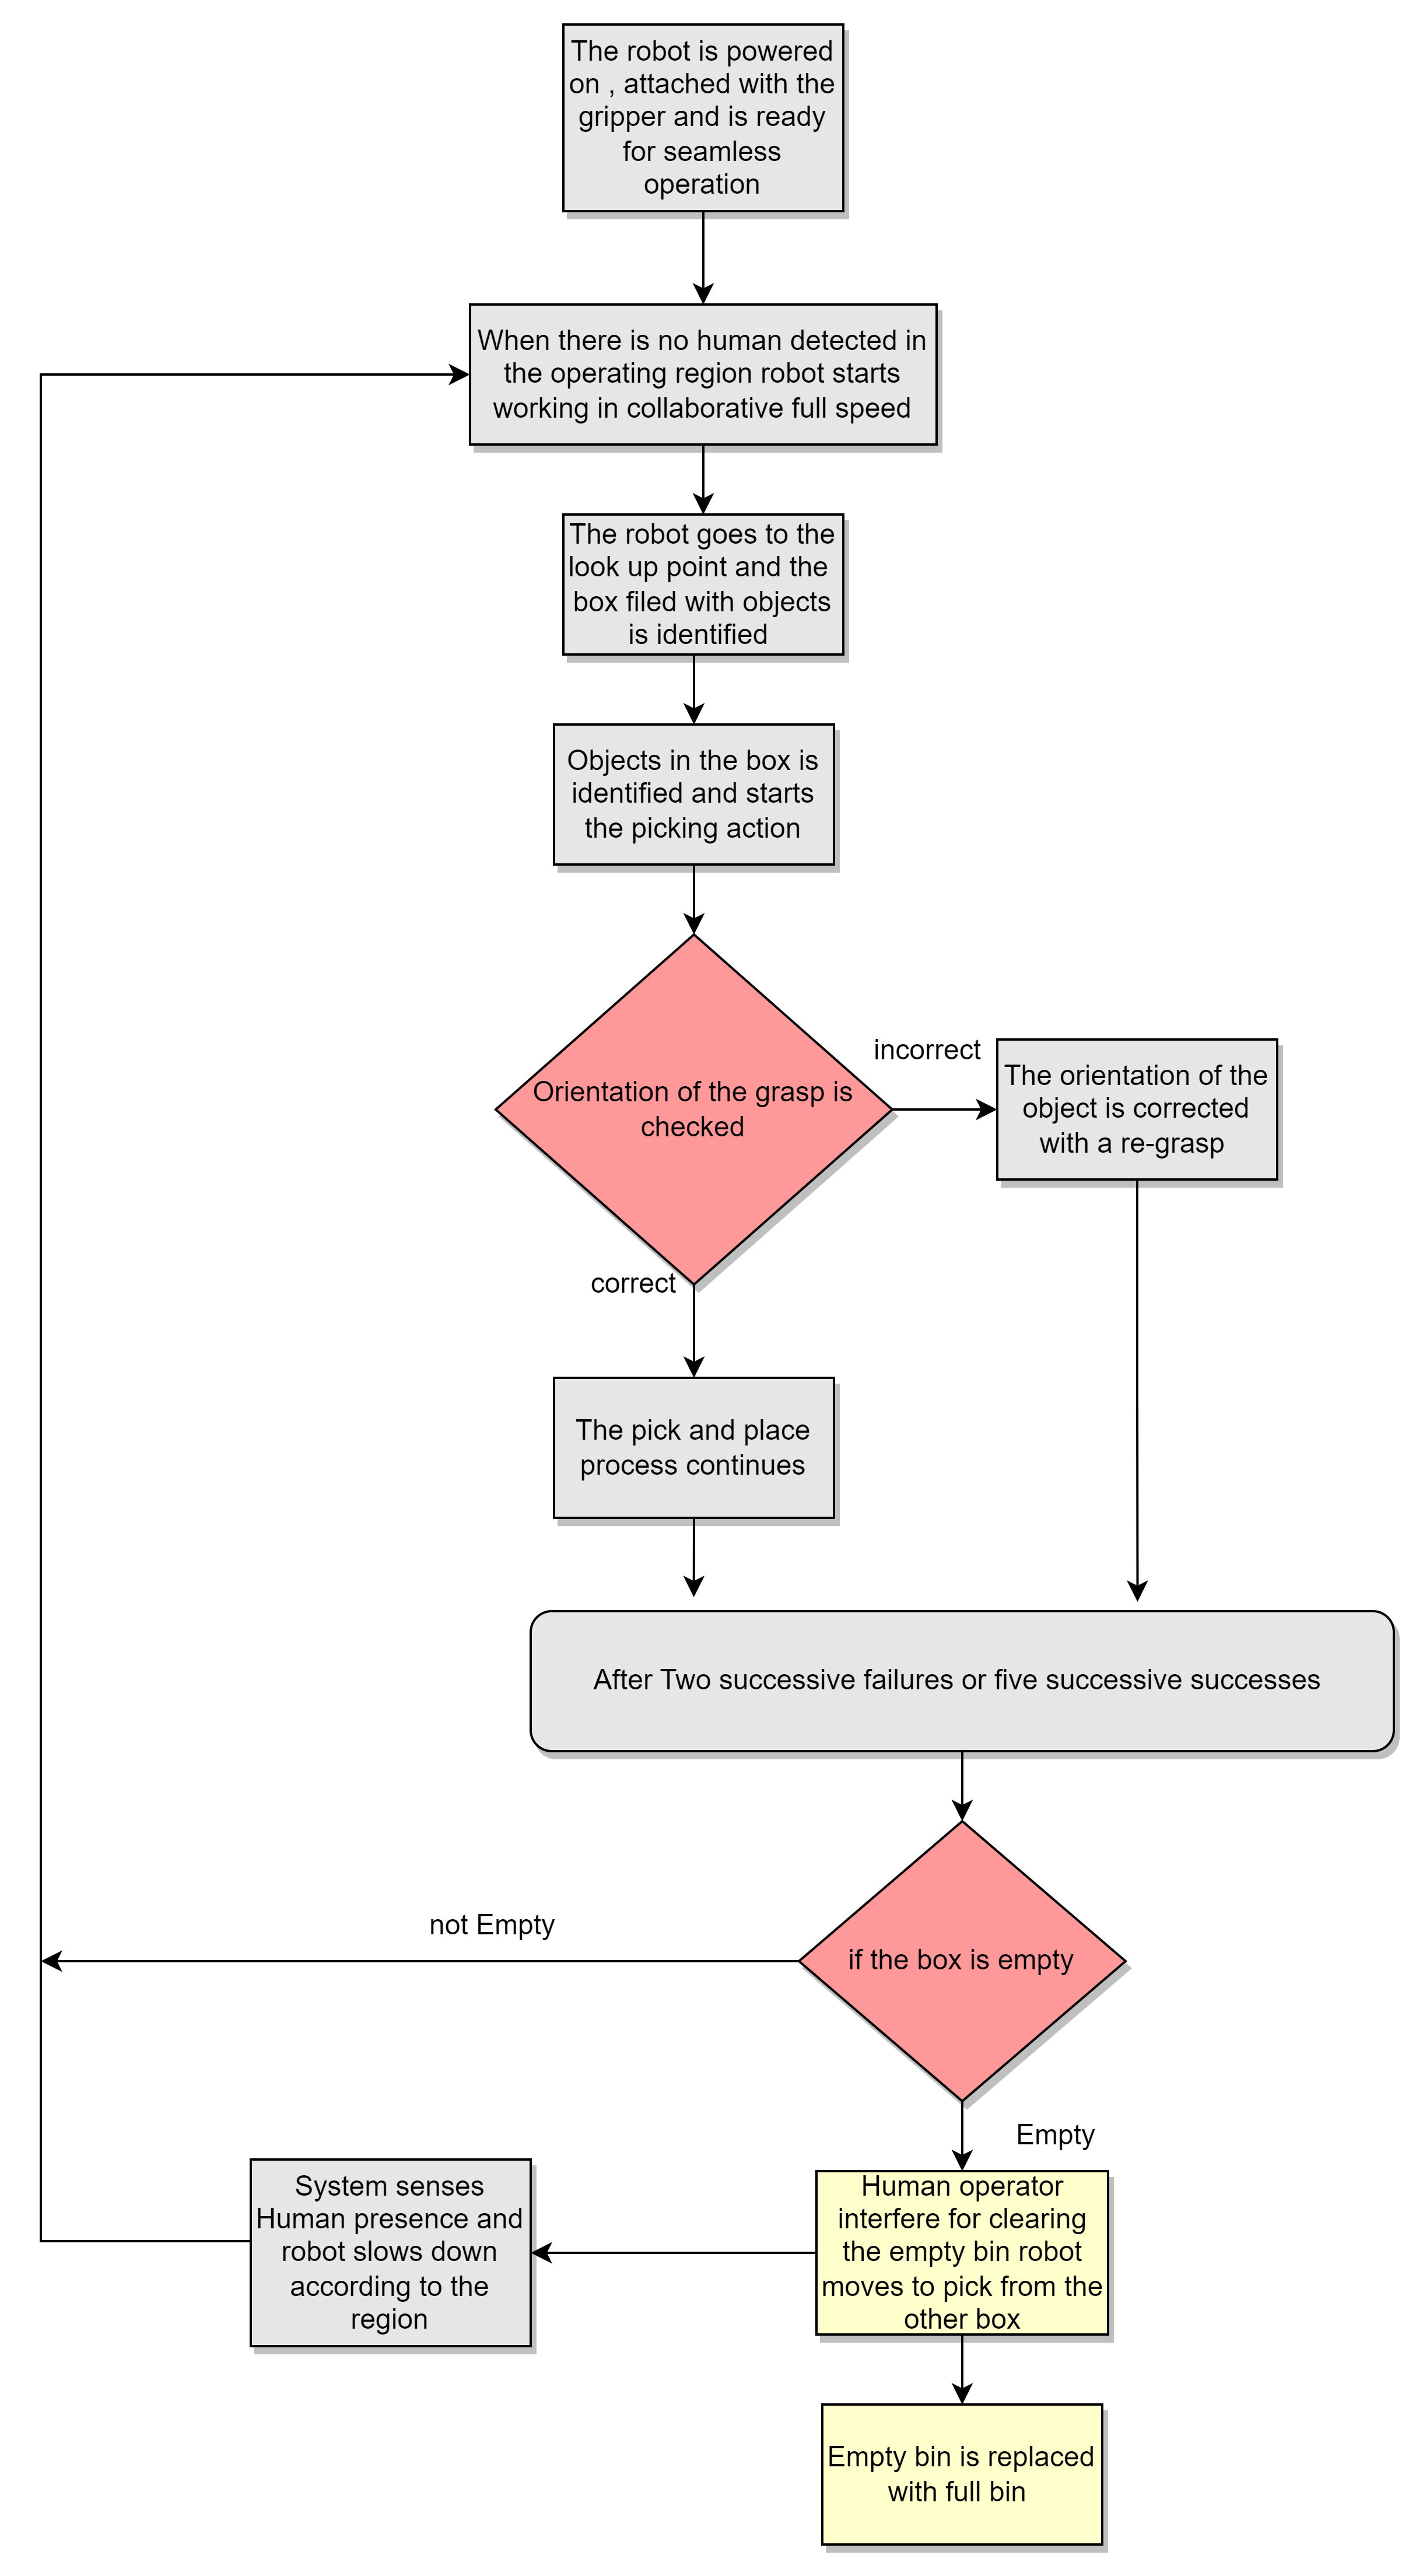
\includegraphics[width=0.5\linewidth]{Figures/SOP_flowchart.png}
    \end{minipage}
    \label{fig:enter-label}
    \caption{Flow chart of the Standard Operating Procedure}
\end{figure}

The bin-picking robot system integrates state-of-the-art components to deliver a reliable and precise solution for the automated handling of machined parts. The combination of a magnetic gripper, RGB-D camera, and Safe Human Detection sensors ensures efficiency, safety, and adaptability. The system's ability to manage potential failures and periodic lookups contributes to its overall robustness and reliability in a manufacturing environment. Regular maintenance and adherence to safety protocols are crucial for optimal performance.

 \subsubsection{Control Structure}

In this system, there are two computers, one would be processing the AI inputs and then sending signals to the other computer which would control the robot with the software. The AI computer after recognizing the object would send the coordinates of the detected object to the control computer. The calculation of the forward and inverse kinematics is done inside the second computer in this case, and the optimal way of approaching the workpiece is found out using this.
The AI computer also sends information about the force to be used by the end effector to pick the object according to the object identified. The Robot-Human interface allows feedback from the operator as well as helps the robot to send signals about its actions.
The number of successful picks and the successful failures are being monitored for this particular application to trigger the movement of the robot to look up point.

The orientation of the pick is monitored, if the orientation is not as expected, then the robot puts back the workpiece. If there are two failures in pick, and then the robot puts back the workpiece the robot has to go to the look up point , There are control triggers from the AI system in these two scenarios

The control unit would have the state and orientation of the robot which is being updated in every one millisecond by the heartbeat signals.
There are passive safety controls like collision detection and safe torque ON when the robot detects anomalies in the voltage behavior and the external forces.
The Safe Human Detection sensor senses the human or any obstacle inside its perimeter and then the robot slows down or the robot stops according to the region where the human is detected the Safe Human Detection sensor is connected to the Digital input of the system. 
As soon as there is an obstacle in the region the Safe Human Detection sensor sends the signal high into the Digital inputs and then the processor first assesses the state of the robot and then asks the robot to slow down or to stop or to be in stop mode according to the state of the robot. 
The monitoring of the robot limits cartesian space and the joint space is continuously happening. This is also limited according to the present ISO standards and technical specifications for the safe operation and integration of robots.





%The limits of the robot are set optimally for the three cartesian coordinates and the orientation of the tool center point to the base and joint space are limited for safety purposes, thus unexpected rotation of the robot arm will not happen, even when the robot is in hand guiding mode.



 \begin{figure}
     \centering
    \begin{minipage}{1.0\linewidth}
     \centering
        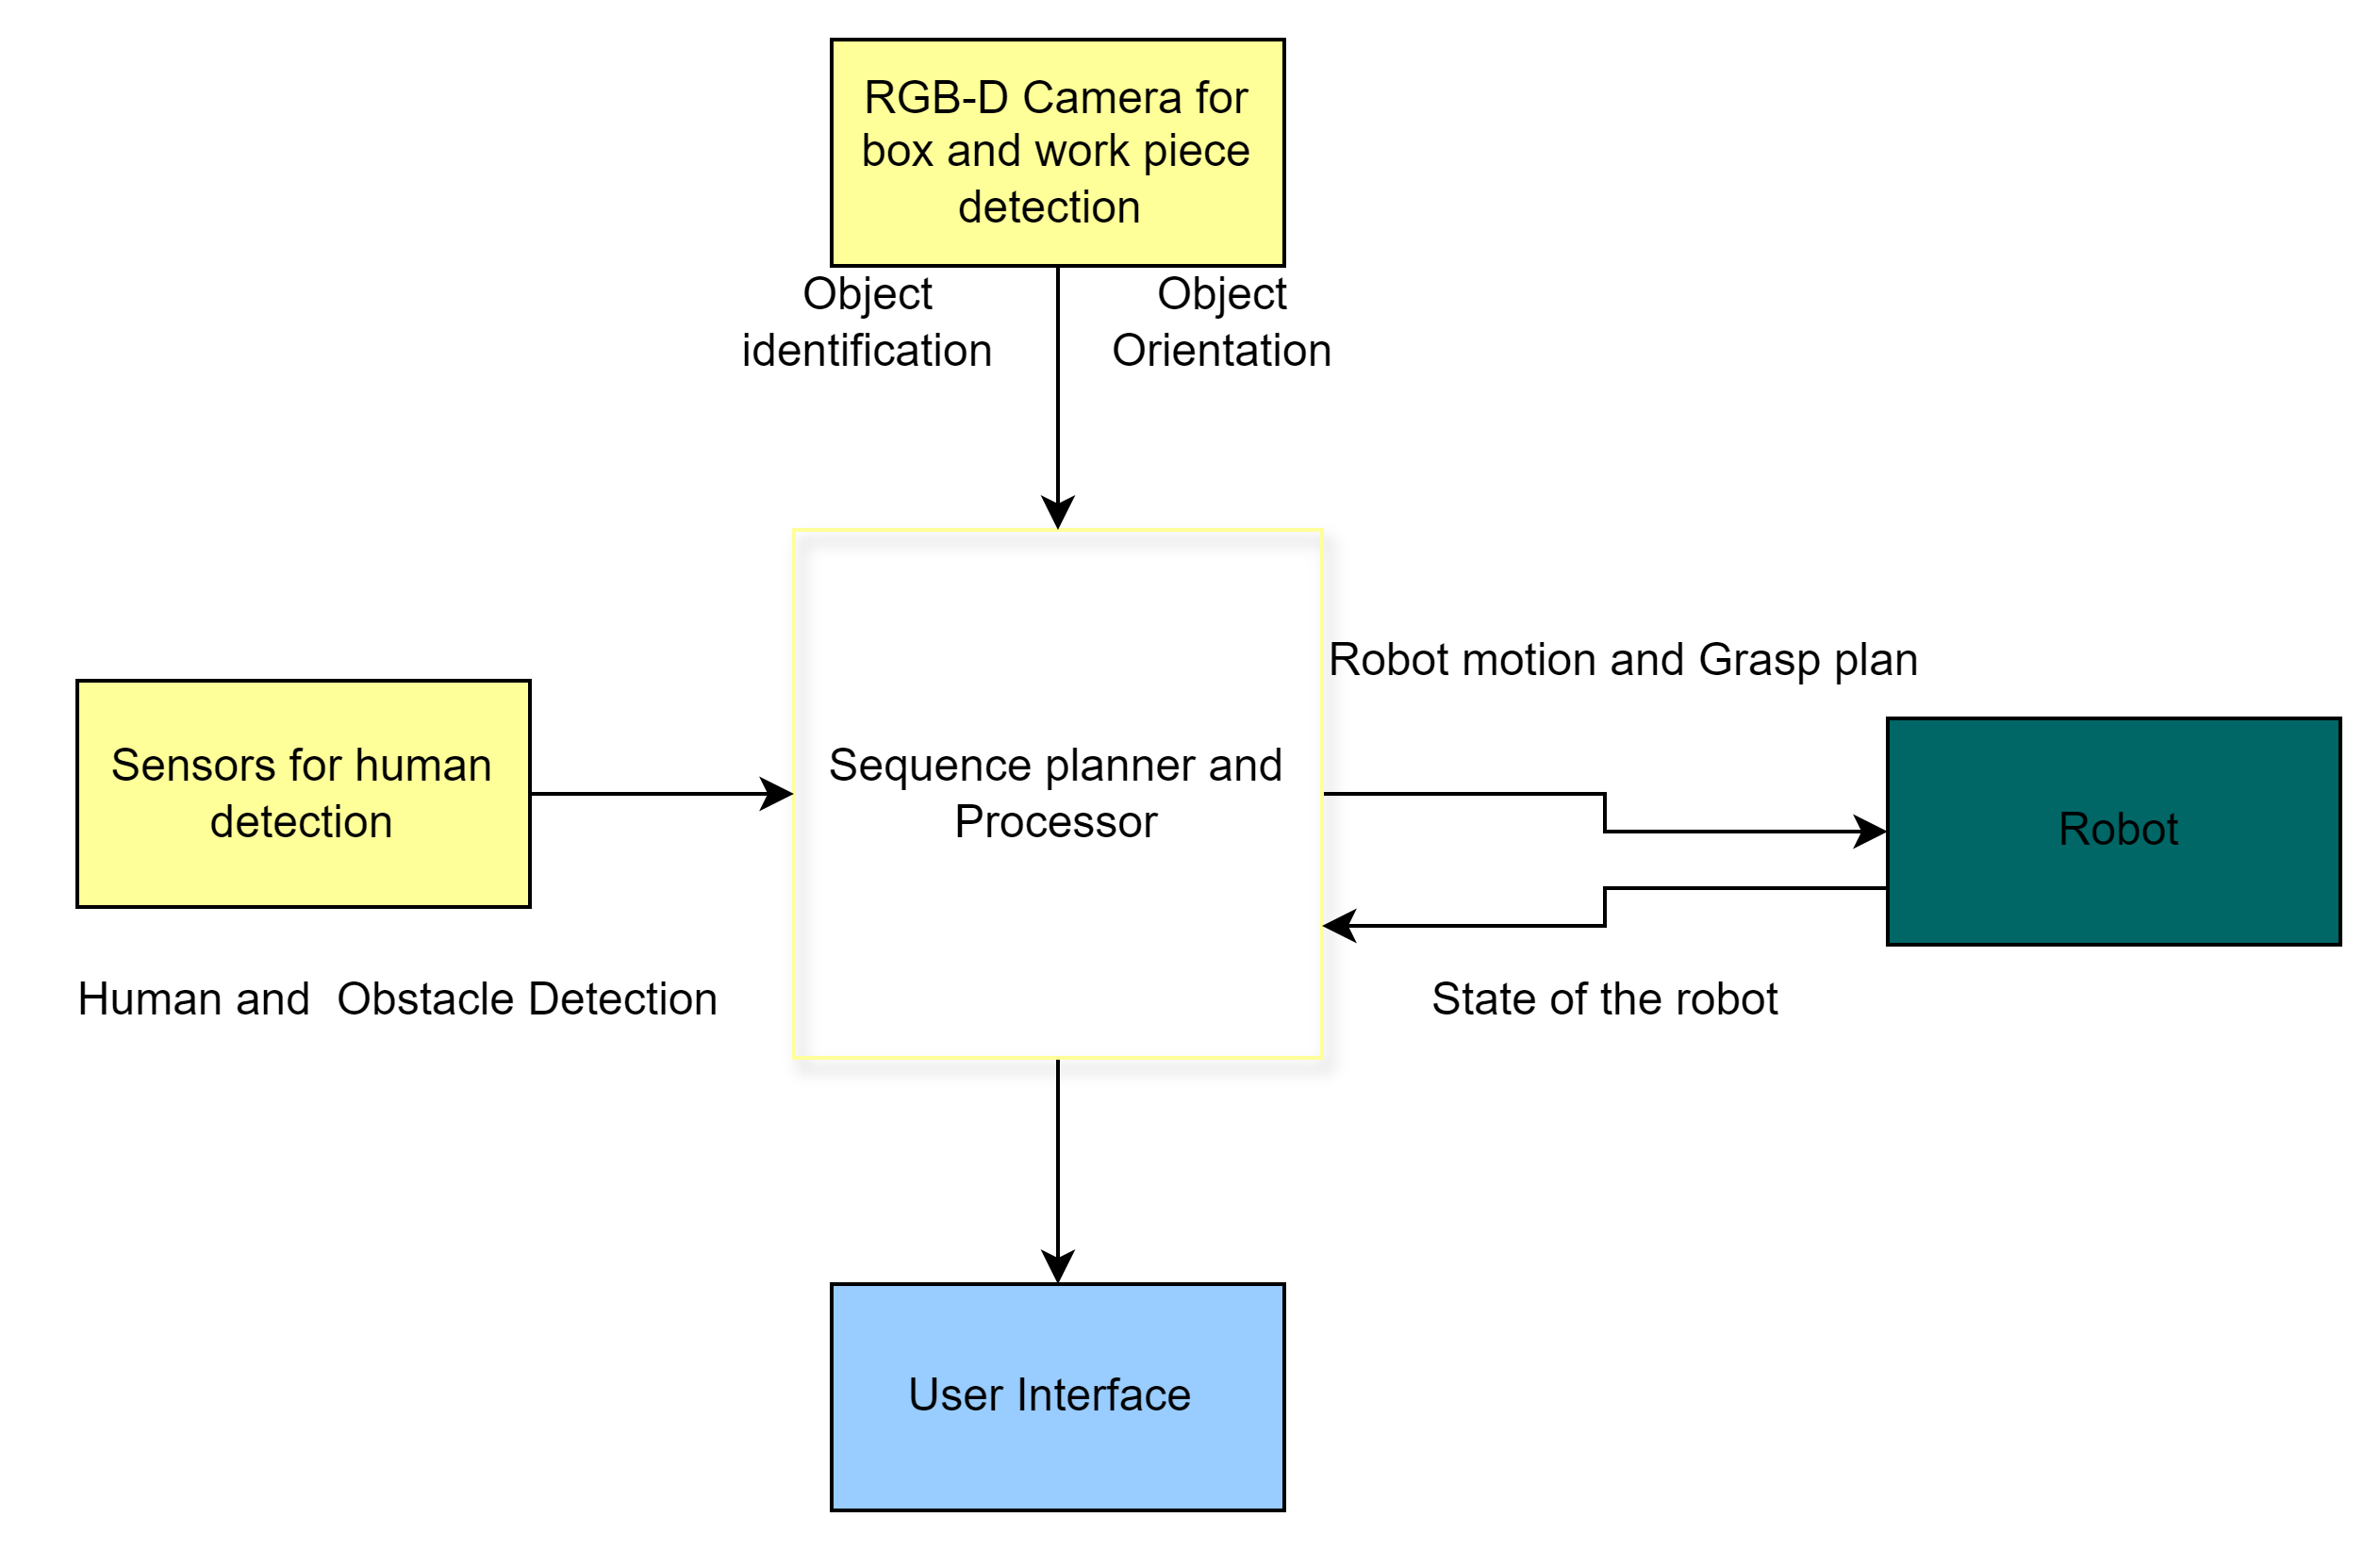
\includegraphics[width=0.75\linewidth]{Figures/Control_Structure.png}
        \centering
     \caption{Control Sequence:Inputs from sensors,processing and output}
     \end{minipage}
     \label{fig:enter-label}
 \end{figure}
 

\subsection{\RaggedRight Risk Assessment Methods and Tools }

 The ISO/TS 15066 or EN ISO10218-1:2011 and ISO 10218-2:2011 do not specifically  dictate a special risk assessment method. ISO 12100:2010 suggests a task-based risk assessment methodology to determine the performance level required for the safety functions.
 
 To enhance the system and process safety there are many techniques available such as FTA, ETA, HAZOP, FMEA STPA, etc. 

Fault Tree Analysis (FTA) is a top-down risk analysis method that examines an entire system by breaking it down to components and analyzing the conditions that may lead to a predefined problem. This problem is called the top event. Defining the top event, decomposing the system into individual components. Identification of relevant events and conditions, and establishing the logical relationship are the main steps of FTA. FTA allows quantitative and qualitative analysis. The result of the analysis is documented using the Fault Tree diagram, illustrating the logical relationship and the need for improvements in the system safety measures.

Hazard and Operability Studies (HAZOP Studies) are a risk analysis technique for a defined system, identifying potential risk in operating and maintaining the system and external risk sources like environmental hazards that can trigger risk for the system itself.

Then we have risk assessment techniques like Failure mode effects (FMEA) which break down the system and analyze the risk of each of the components or each step of the process. 

System Theory Process Analysis (STPA) is a comparatively new risk assessment tool that can be used to study the control structure of the system, how the interactions between the components are processed, and analyze if there are unsafe control actions.

FMEA and STPA are discussed further in the next subsections as we are doing our risk analysis of the AI-integrated robotics system using an extension of FMEA with STPA




\subsubsection{\RaggedRight Failure Mode Effects Analysis }
FMEA is an engineering analysis method to be used to analyze the system from bottom to up for the design of new systems, 
 new processes, new software, and later to improve production and design. It is useful to evaluate failures that may occur, the effect of the failures on the system, and mitigation strategies. EN IEC 60812:2018 is a standard that specifies how to use this risk assessment tool effectively in the industry. This standard illustrates use of FMEA in different scenarios. 

FMEA applies to hardware, software, and human action interface between humans and hardware or software in any combination. This could be used in any stage of the lifecycle of a product, process, or system. It is based on the reliability theory.

The four stages of FMEA are preparation, risk identification, risk assessment, and risk reduction. The preparation stage is where the boundary conditions are explained the process flow chart is drawn and most importantly the decisions about what should be included and excluded are considered. Risk identification starts by identifying and describing the function of relevant steps in the process and each item's potential failure modes. Risk assessment could be done by finding the RPN and estimating the likelihood of failure. Risk reduction is the step where corrective actions are developed and implemented.[30]

The analysis starts from the lowest component and proceeds up to the failure effect of the overall system. A failure effect of a lower component can be a failure mode for a component at a higher level. The potential problems in the design and development of the system can be studied.

There are different applications for the FMEA considered such as the software FMEA and the process FMEA. The software FMEA can be used on embedded real-time systems. Software FMEA is a very important failure analysis method since the software does not fail randomly and all the software failures are systematic failures, due to wrong specifications or requirements of the function.

In this analysis, each failure mode portrays the potential failure of the product or system and these failure modes' cause of the failure and the effect of the failure are entered in the spreadsheet called the FMEA table. 

In this research, we use process FMEA to analyze the process, where the robot is used to pick and place the workpiece using integrated artificial intelligence. We break down the process into steps and substeps and do the analysis 
 
 The integration of Artificial intelligence in robotics introduces a paradigm shift that brings several risks into the scenario. We use FMEA as our risk assessment tool and not other tools like HAZOP, Fault Tree Analysis, Event Tree Analysis, or Common Cause Failure Analysis because of its unique features.
  
  FMEA is useful in identifying causal factors such as interface errors, Hardware and software interaction, and software defects in the usage of improper protocols or even the architectural mistakes in the software of the system.
 
 FMEA allows the breakdown of the system into constituent parts so that the identification of risks is possible at the component level. In the context of AI in robotics, it is essential to break the system into constituent parts as there are many intricate algorithms and dynamic decision-making processes in the control system.
 
 The proactive nature of FMEA also was a reason for us to choose this risk assessment tool. The other risk assessment tools use the reactive method after the occurrence of the risk. This is suitable for dynamic environments and real-time decision-making.

FMEA allows quantitative and qualitative analysis of risk. The severity, occurrence, and detection of the failure modes contribute to the quantitative analysis of the risk while the team's expertise and experience could add qualitative insights. 

FMEA allows cross-disciplinary collaboration, experts from robotics, Artificial Intelligence experts, other engineers, and domain specialists. This allows views from different angles to a problem and could lead to more robust risk reduction. The algorithmic biases uncertainties in learning and adaptability to complex situations can be tailored using FMEA. 

FMEA encourages the thorough documentation of the risk assessment processes. The documentation is invaluable to trace back the actions taken. This documentation is also essential for the certification processes. In the rapidly growing field of AI, having a well-documented risk assessment methodology is essential for presenting in due diligence of the AI-based control systems.

FMEA deals with the known potential failures and introduces new countermeasures to mitigate the negative effects., it is hard to identify all risks in the early phase of the development using FMEA. Especially for intelligent control systems that may make their own decisions.



\subsubsection{\RaggedRight System Theoretic Process Analysis }

System Theoretic Process Analysis-(STPA) is a top-down proactive method for analysis that is based on the System Theoretic Accident Model and processes. This is a relatively new method of risk analysis that is beyond directly related to failure events or component failures but to more complex processes and unsafe interactions among system components.This analysis is mentioned in ISO 21448:2022 which addresses functional insufficiencies of systems.

STPA uses a model of the system that consist of a functional diagram of the control system not really the physical parts in the control system but how the interactions are being worked.

STPA also includes Planning, which means defining the purpose of the analysis including the definition of the system, and boundary conditions. Identifying system losses and hazards. The second step is creating a hierarchical diagram of the control structure. The third step in STPA is an analysis of the control actions. The next step includes describing the causal factors that can include unsafe control actions and hazards, translating uncontrolled actions into constraints on the behavior of each controller. The unique features of STPA enable the risk assessment of the control systems.

STPA defines hazard as the state of a system or condition that could lead to an accident. Since an inadequate control action can lead system to a hazardous state . STPA studies whether a control action required is provided, if the control action provided is safe if the control action being provided in wrong time or sequence and if it is provided in inadequate timing.

In this study of the control actions we consider communication failure for example delayed failure or corrupted communication inside the system since the delivery of the control command to the component from the processor is also an important aspect of this.



The systemic approach in which the whole system is considered and the interaction between the components is analyzed rather than doing risk analysis on individual components. It helps in the holistic concept of the system and the potential vulnerabilities of the system.

STPA analyses the processes inside a system. The hazards arise from interactions of the components inside the system which allows a nuanced understanding of the system working.

The proactive approach of STPA allows the early detection and identification of potential hazards, which allows for the prevention of the hazard being embedded in the system in the development cycle itself.

The strong emphasis placed on control systems by STPA examines the working of the control system and identifies the deviation from the correct working of the system. This in turn helps in identifying enhancements in control measures.

STPA not only considers technical aspects but also takes into consideration the human factors and organizational factors that could cause hazards. This helps in a holistic approach to risk assessment which could include technical and human-related risk.


The causal analysis method employed by STPA allows to identification of root causes for the potential hazard which could help in more effective mitigation of the risk from various factors contributing to the risk.

STPA is being adapted in different fields like the automotive and aerospace industries for risk assessment in intelligent control systems. This could also be used in the field of robotics.

STPA considers hazards as a challenge in managing system controls, encompassing not just failures but also hazardous successes. This implies that even if individual components operate successfully, their combination may still result in a loss of system integrity. As a result, STPA is frequently utilized in safety-critical systems and scenarios where the most severe outcomes need to be anticipated.

A notable limitation of STPA in risk assessment is that we cannot quantify risk using STPA for example there could not be an RPN number if we use STPA for risk analysis.

\subsubsection{\RaggedRight Risk Assessment using FMEA-STPA } 

The purpose of this project is to conduct risk assessment for the perception-based grasping system in robotics. The analysis aims to identify, evaluate, and address potential failure modes in the perception components, algorithms, and related processes to enhance the safety, reliability, and performance of the grasping system. This may include Assessing the Sensors, Object Recognition Algorithms, Environmental conditions, Integration with the Grasping mechanism, Communication, and Data processing and how this might affect human-robot interaction.

For risk assessment of the AI systems in robots, we use the tool FMEA with an extension of STPA, which is strongly advocated by the authors of \cite{author30}. To overcome the limitations of both the tools we use this extension. We use a brainstorming session for the effect cause analysis of the identified potential use case.

For FMEA which is a bottom-to-up risk assessment strategy we study each component in the process and for STPA which is a top-to-down risk analysis we study every interaction of the components in the system and the risk assessment according to the recommendation of the standard EN ISO 10218-2:2011 for robotics systems which suggests a structured risk assessment. Since it is difficult to find out the occurrence and detection of intelligent systems we use STPA for the controllability of occurrence and detection using.

The tool complements the shortcomings of each other. For example, FMEA is component-centric or event-focused, this can lead to dangerous success meaning even if the components are not failing the whole system working together can cause a failure leading to a hazardous event. this can be monitored using STPA which identifies the risk at the system level or according to the process.

While FMEA gives the prioritized actions for the mitigation of risks. STPA gives safety requirements to be followed based on technical and human aspects of the system. The integration of these tools could be a better way to assess the intelligent complex systems

The process requires a well-experienced system engineer, robotics engineer, AI specialist, a Product manager who decides the requirement for the system, and A Functional Safety expert as the first step of the risk assessment.


We try to quantify the severity, occurrence, and detectability on a scale of 1 to 5. We use the STPA and the definition of the control structure for identifying unsafe control actions.
It is crucial to tackle a particular type of risk arising from uncertainty, as responses or inputs/feedback can be appropriately supplied at the right moment (neither prematurely nor belatedly). The combination of these methodologies the advantage is FMEA gives the potential risk of failures in process aspects and the STPA gives the potentially unsafe control actions that could influence the acting decision of the system. 
Thus when we quantify risk , we think the logic, if there are control actions for a particular error arising due to malfunction of the components, the occurrence rating would be less for this error, which can lead to a failure, Similarly if there is no control for a particular failure, the occurrence rating would be very high. This is similar in case of detectability also. Thus STPA is relevant in the risk assessment of the intelligent control system which give inputs for the robot actions.

 However, this entails inherent uncertainty, especially when utilizing machine learning techniques. For example, when the vision system furnishes information to the control system regarding the operator's position, the algorithm may exhibit uncertainty regarding the precise position, particularly if the human is partially obstructed. This uncertainty will place restrictions on when the control system can carry out an operation. In the brainstorming session, these failures arose from uncertainties that were considered, and the possible remedies were discussed. 
 

\vspace{0.5cm}
\subsubsubsection{ \textbf{Failure Modes}}
\vspace{0.2cm}

When we do the Failure modes effect analysis for the process each step of the process is considered and the failure modes are determined. Each step of the process is then subdivided and failures are determined.

\begin{figure}
    \centering
    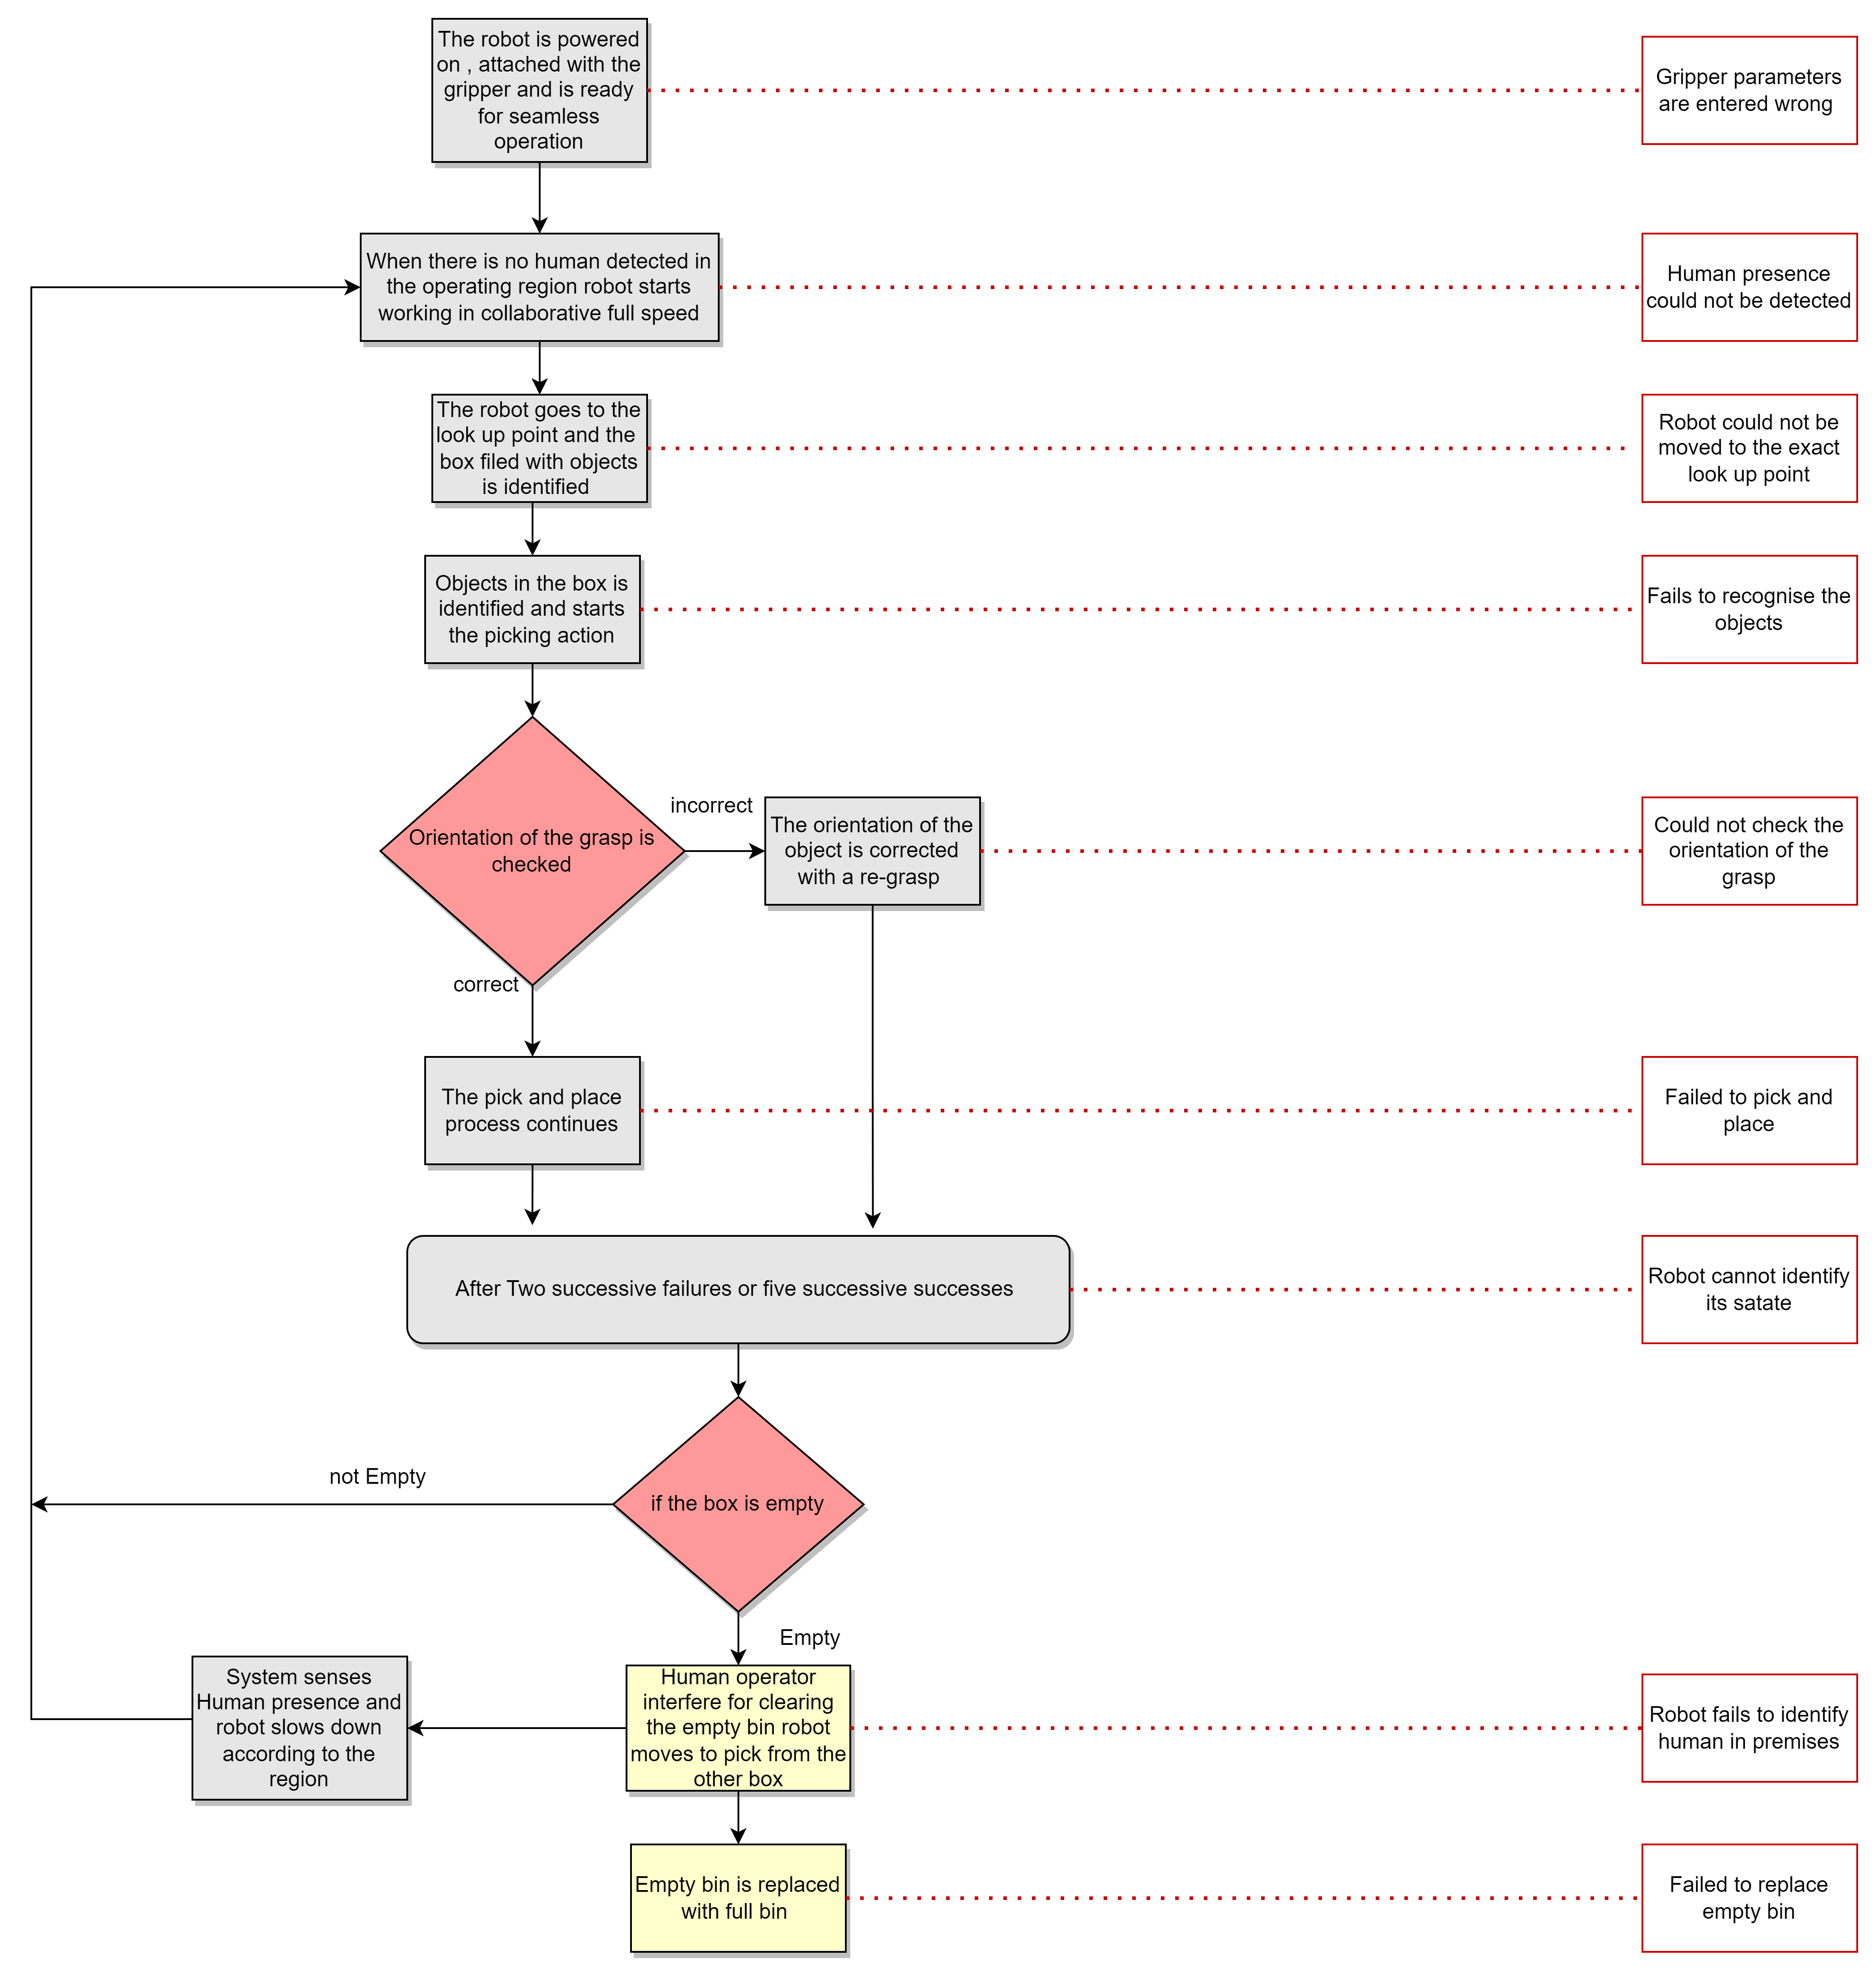
\includegraphics[width=1.0\linewidth]{Figures/Failure.png}
    \caption{Failures Identified in Standard Operating Procedure}
    \label{fig:enter-label}
\end{figure}

So when we consider the industrial use case for grasping it can be divided int 4 major phases which can be subdivided into steps for the FMEA, which are Object Identification Phase, the Picking Phase, the Placing Phase and the Human intervention phase.

We can divide the  Object identification phase into substeps like Object detection, Object identification, and Grasp Estimation.
The following failure modes could arise in the above phases.

1. False positives: The system detects objects even if the bin is empty.

2. False Negatives:  The system is unable to detect objects inside the bin even if there are objects inside the bin.

3. Over-segmentation: Here the system takes the input and can see one object as two or more due to over-segmentation.

4. Under-segmentation: Here the system takes the camera or sensor input and sees two or more objects as one due to under-segmentation.

5. Occlusion: The system is unable to recognize the objects that are occluded due to the objects above in the box.

6. Incorrect Identification of Object: The system could incorrectly identify the objects and may damage the object due to this.

7. Incorrect Orientation Recognition of Object: The system incorrectly recognizes the object's orientation.


The second phase can be divided into substeps where the robot moves to pick the object, the robot applies the correct force to pick the object and then finally grasps. In this phase after grasping the robot checks the orientation of the object after grasp.
The following failure modes could arise in the above phases.

1. Incorrect Orientation of the Gripper to Pick the Object: The gripper is oriented incorrectly, which could cause the pick of the object incorrectly.

2. Incorrect force for pick.

In the 3rd phase, the robot places the object and this can be subdivided into the moving phase where the robot holds the object and moves to the final destination, and the placing phase in which the robot places the object in the required orientation.
The following failure modes could arise in the above phases.

1. Objects could be misplaced on the conveyor belt could cause damages

2. Misalignment of the robot arm during the process




Human intervention is asked, whenever the box is empty for replacement. In the Human intervention phase for replacing the bin the following failures could happen, the Safe Human Detection sensor is used for detecting human approaching and the outputs would be different as there are zones for the human to interact with the robot.
The following failure modes could arise in the above phases.

1. False negative in human identification: The system fails to identify the human presence near the system

2. Human Location Uncertainty due to Occlusion: The system identifies to detects human presence but cannot identify the exact location of the human due to Occlusion

3. Delayed Human Detection: This can cause great danger for the operator, this is a severe failure mode where there is a delay in human detection due to communication breakdown between sensors and processors or high computing time for the processor. 

\vspace{0.2cm}
\subsubsubsection{ \textbf{Control Analysis}}
\vspace{0.2cm}

%In addition to problems caused by the failure of specific functions or components, interactions or control problems between system components are considered as hazards, and are effective in identifying the hazards based on unsafe control actions between components


We do a Control Analysis, to understand the communication control actions and the feedback loops between the AI system and the robot control system. The first phase of the analysis is the assessment of the clarity, reliability, and efficiency of data exchange.

The analysis also includes whether there are control actions provided, not provided or provided with timing discrepancies. This assessment may help to find out the vulnerabilities of the control mechanism. The timing discrepancies mean if the control action lasts too long, if the control action stops prematurely if it happens too early, or if it happens too late.

One of the major control actions in this use case is the robot reducing its speed as soon as the system detects a human in the virtual cell where the robot is working and, when the human operator is in the second region inside the collaborative workspace that is very close to the robot, the robot stops all its movements. This action starts at the moment the human steps inside the region and lasts long till the human is moved out from this region. This is one of the active control mechanisms which is used to avoid collision between the operator and the robot.
Detection, Evaluation and Identification of the box and the objects are control actions which is provided just before the pick is started 

The trigger to pick and place the object. The other control action is providing the required force for holding the workpiece by the magnetic gripper. As soon as the object is identified and the robot is near the object for pick. the magnetic force should be provided for the pick. This would last till the object is placed in the correct place.

Changing the states of the robot and the whole system is an action provided by the control systems from its inputs.  When analyzing the system's change of state for some of the potential failure modes we found that, there is a lack of control action thus limiting the dangerous success of the robot operation. Thus few of the control actions are recommended to be implemented for the perception-based pick-and-place robotic system.

These are the implementation of fail-safe mechanisms and predictive maintenance and analysis of the sensors on the robot and the sensors in the surroundings. This is discussed in detail in the next chapter. The need for planned safety also arose from this control analysis a small description for the need for planned safety is described.

In short, this control analysis also helps to analyze the interactions between the components, which helps in finding not only the failure of specific components or function of the robot but the unsafe control actions too.

\vspace{0.5cm}
\subsubsubsection {\textbf{Uncertain Failures}}

The uncertain input controls from the vision system and the sensors on the robot and the application environment reduce the trust in the system. This also acts as a barrier for the system to reach the required performance level with safety. 

The uncertainty in the position of humans or any obstacle in the robot's path or in the surroundings should be reduced. The uncertain events and the events with no control preventions are identified with this process.

To implement the planned safety, this is important. An approach of planned safety and active safety together is essential for the robot system integrated with AI to mitigate unknown risks thus a deliberative safety implementation is used by the control software of the system thus the unintended signals would not be produced by the control system.  Planned safety is an approach defined by the researchers [35] for integrating intelligent human-robot collaboration in Industry 4.0. This approach helps in rectifying the uncertainty from the vision system and other sensors used in the system.

%We found the major failures for the use case after compiling all the steps involved in the process and then breaking down the process according to the SOP. as Sensor Malfunction, Object Recognition Errors, Communication Breakdown, Environmental Changes, Algorithmic Errors,	Human Interference, Calibration Issues, and Safety Violations.



%The Effect-Cause Analysis is done for the identified failures also done in the brainstorming session



 
\subsubsection{\RaggedRight Decision Criteria for Treatment of the failure modes }

The Decision criteria for the treatment of the failure modes are based on various factors such as the severity, controllability, and probability of detection other factors like complexity integration of the treatment action to the system and the effect on the performance matrix are also considered in the decision criteria. The risk matrix is found  out of the severity, occurrence, and detectability found in the table.

Here severity is assessed by taking the potential failure effect into account. We use a five-point scale for this. The reasons and the failure mechanism is also noted down in while severity is being checked

\begin{table}[ht]
\centering\
\begin{tabularx}{\linewidth}{|X||X||X|}
\hline
 Rating & Description & Criteria \\
\hline
1 & Very Low &  Objects not picked correctly \\
\hline
2 & Low & compromise in cycle times, Objects not placed correctly \\
\hline
3 & Moderate & Robot colliding, damage to the workpiece, damage to the obstacle\\
 \hline
4 & High &  Damage to the robot, System shutdown\\
\hline
5 & Very High & Injured Operator, Fatality\\
\hline

 \end{tabularx}
  \caption{Severity Rating (S) Table}
\end{table}

While analyzing the probability of the occurrence and detection the usage of the STPA comes into the scenario where we analyse whether there are control actions provided for this potential failure mode, if the control action is provided if it is sufficient, and if it is efficient. 
    
The probability of occurrence is taken into account considering the system's complexity, potential failure mode, and cause of failure which is also in a five-point scale. The uncertain control actions are also mentioned in this part of the table. If there are no control actions provided for this from the system the maximum occurrence rating would be assigned for this cause of failure mode.

Thus instead of quantifying the failure rate we consider whether the control action provides prevention from the failure and based on the provision of the control action and based on the efficiency of the control action we try to number the control prevention. If there is suitable control prevention to protect against potential failures, then it is given 1 and if there is no control prevention at all then it is numbered 5. The occurrence rating  from 2 to 4 is assigned based on the suitability and length of the control action provided.


\begin{table}[ht]
\centering\
\begin{tabularx}{\linewidth}{|X||X|}
\hline
 Rating & Criteria \\
\hline
1 & Suitable and Efficient Control Provided \\
\hline
2 &  Suitable Control prevention for prolonged time   \\
\hline
3  & Suitable Control Prevention but wrong timing (too early or too late) \\
 \hline
4  &  Suitable Control Prevention but  for short time \\
\hline
5  & No Control Prevention \\
\hline

 \end{tabularx}
  \caption{Probability of Occurrence Rating (Po) Table}
\end{table}

Detectability is assessed on a five-point scale based on the complexity of the component and the potential cause of failure. The detectability is also measured by the ability of the processing unit to detect whether there are potential failures for the intended functionality.

If there is no detection of the cause of failure then the probability of detection value would be considered the highest. If there is suitable detection for the cause of failure then it would have the lowest rating. 

\begin{table}[ht]
\centering\
\begin{tabularx}{\linewidth}{|X||X||X|}
\hline
 Rating & Description & Criteria \\
\hline
1 & Almost Certain Detection & Detectable at least 90 percent of the time of failure \\
\hline
2 & Highly likelihood of detection &   Detectable at 75 percent of the times of failure\\
\hline
3 & Moderate &  Detectable at 50 percent of the times of failure \\
 \hline
4 & Low likelihood of detection & Detectable at 25 percent of the times of failure  \\
\hline
5 & No Detection & Detectable at less than 10 percent of the times of failure \\
\hline

\end{tabularx}
  
\caption{Probability of Detection Rating (Pd) Table}

\end{table}


Later the Risk Priority number (RPN) number is calculated by multiplying the Severity value by the Probability of occurrence times the Probability of Detection.

According to the RPN obtained for the failure modes we prioritize the mitigation methods to reduce the risks with the highest RPN. The categorisation of the RPN is explained in the next section
The mitigating actions proposed should bring the risks to an acceptable level. Active safety and planned safety approaches can be used to bring down the risk to a minimum.

After the reduction of the risk, the process can be iterated to identify new potential failures and risk reduction methods. The SOP should be altered in such a way that these process failures are mitigated if needed or the system requirements should be changed in order to reduce the RPN thus the detectability and the controllability of the very severe risks can be brought down.

The major results of the risk analysis were the implementation of the control actions for the potential failure modes, including upgrades in the sensors used, and the introduction of predictive analysis algorithms for the sensors, thus detecting anomalies in the sensor behavior. This is explained in the next chapter.




% 1. Partition the system to be examined into subsystems and components, taking the
%architecture of hardware and software into account.
%2. Assign the application function to each component. In this step, functional and nonfunctional requirements have to be interpreted.
%3. Determine and analyze the potential failure mode, cause of failure, and failure effect
%that can lead to a hazardous state. For instance, the failure mode “false break activation”
%could have the cause of a defect in the SW of pressure determination and the effect
%of a potential crash situation between two cars. Another example regarding security
%is, for instance, a failure or threat mode classifying the way in which vulnerabilities
%are exploited (Schmittner et al. 2014). A threat mode could be “attacker is pretending
%to be a measurement device” violating the integrity of the system. The cause could
%be an encryption problem or security breach and results in “system is unreliable and
%potentially unsafe.”
%Each failure mode represents potential product failures that can occur. Failure mode,
%cause, and effect are entered in the spreadsheet fields related to the appropriate component and function. The causal factors are associated with software defects, interface
%errors (architectural, protocol), HW/SW interaction (signaling), reliability, security, and
%real-time constraints. The potential failure effects could be the following: risk of collision, the operator is not alerted, a potential crash situation, or the authorization of
%external hackers to manipulate the collision avoidance system.
%4. Evaluate risk and calculate the risk priority number (RPN). To calculate the RPN as
%described by McDonald et al. (2008), the severity of the %of their occurrence, and the detectability of the failure causes have to be assessed first.
%The abbreviations used below for severity, probability, and detectability, i.e., B, A,
%and E, are adapted from the study (Mackel ¨ 2001).
%– Severity (B): The severity value is assessed taking the potential failure effect into
%account. A five-point Likert scale is used, ranking the impact from 1 (no impact)
%to 5 (catastrophic, i.e., potential crash situation)
%– Probability of occurrence (A): To assess the probability of occurrence, the complexity, the potential failure mode, and cause of a failure have to be taken into
%account. A five-point Likert scale is used to rank the probability, starting from 1
%(very low, 0.01%) to 5 (very high, 50%).
%– Detectability (E): The detectability depends on the complexity of the HW/SW
%component and potential cause of a failure. A five-point Likert scale is used to rank
%the detectability, starting from 1 (very low probability (0 to 19%) that current controls will detect the cause) to 5 (very high probability (80 to 100%) that current
%controls will detect the cause).
%– Calculation of risk priority number: RPN is calculated by multiplying the values
%of severity, probability of occurrence, and detectability. RPN = B ×A×E, where
%B, A, and E denote severity, probability, and detectability according to above.
%RPN ranges from 1 to 125

%The standard Operating procedure for the use case

%The System flowchart.





  %\centering
 % \begin{tabular}{|c|c|c|c}
  %  \hline
   % Failure Mode & Severity  &  Detectability & Contrallabilty \\
   
 % \end{tabular}




%\subsection{\RaggedRight Safety of the Intended Functionality }
%Refer26
%3.3 Establishment of Process to Reflect SOTIF of Autonomous Driving Logistics Robot
%It is the process according to ISO/DIS 21448 SOTIF standard and Figure 2, and the detailed output is as
%Table 2. Figure 5 shows the procedure performed by SOTIF [12].
%Figure 5. ISO/DIS 21448 SOTIF process
%Table 2. Work products of the SOTIF process
%Clause Work Products
%5 Specification and design - Documentation detailing the specification and design
%6 Identification and evaluation of hazards
%- Hazards at the vehicle level
%- Risk evaluation of hazardous behaviors
%- Acceptance criteria
%7
%Identification and evaluation of potential
%functional insufficiencies and triggering
%conditions
%- Identified potential insufficiencies of specification,
%performance limitations and triggering conditions
%(including reasonably foreseeable direct misuse)
%- Evaluation of the response of the system to the
%identified triggering conditions for their acceptability
%8
%Functional insufficiencies and triggering
%conditions
%- Specification of SOTIF measures
%9
%Definition of the verification and
%validation strategy
%- Definition of the verification and validation strategy
%10
%Evaluation of known hazardous scenarios
%(Area 2)
%- Verification results to show that the intended
%functionality behaves as expected in the known
%scenarios
%11
%Evaluation of unknown hazardous
%scenarios (Area 3)
%- Validation results for unknown hazardous scenarios
%- Evaluation of the residual risk
%12 Criteria for SOTIF release - SOTIF release argumentation
%13 Operation phase activities - Field monitoring process


%Refer [26]
%\begin{figure}
%   \centering
%   \includegraphics[width=0.5\linewidth]{image.png}
 %   \caption{Enter Caption}
%  \label{fig:enter-label}
%\end{figure}


\subsubsection{\RaggedRight Categorisation of Risk Priority Number }

  The risk priority number is considered the highest when the severity X Ocuurence X Detection is the highest possible number that is 125.
  
  Based on the recommendations from the experts in the FMEA  the risk priority number above 75 was considered high risk and there should be appropriate measures taken to ensure the reduction of the risk priority number.

Risk Priority numbers below 30 are considered low risk and the system can have minimal risks, these risks can still be monitored but are of lesser priority.

The Risk Priority number below 75 and above 30 falls under medium risk and this should also have measures taken to reduce the risk but it is not as priority as the high category risks.
